\documentclass[letterpaper]{article}

\usepackage{amsmath}
\usepackage{amsfonts}
\usepackage{graphicx}

\begin{document}

%% testing from desktop

\title{TBD}
\author{TBD}

\date{\today}

\maketitle

\begin{abstract}
	TBD
\end{abstract}


\section{Introduction}

%% testing testing! 
%% testing twice 

TODO: Lagrangian assumption vs kinematic assumption. Investigate what happens when the transformation is non-linear.

\subsection{Define Lagrangian \& Hamiltonian mechanics}

Talk about disippative systems.

\subsection{Derivation}

\begin{figure}[h]
	\centering
	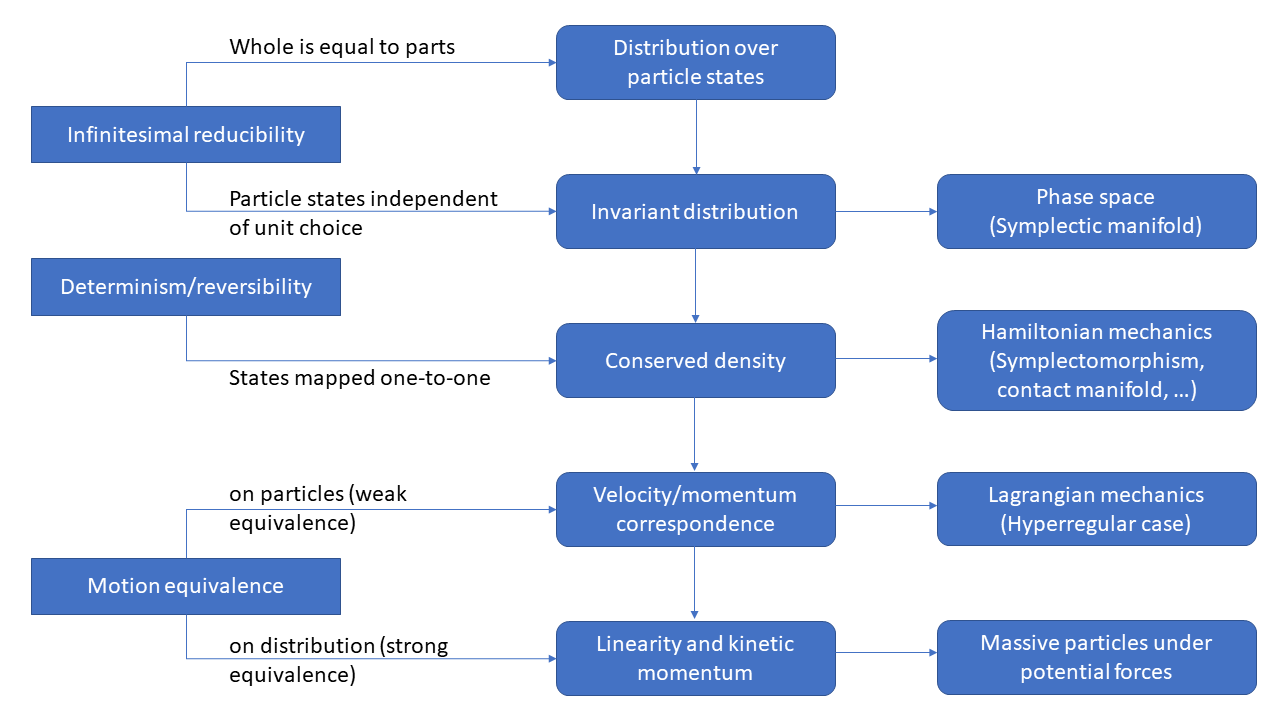
\includegraphics[width=\textwidth]{Diagram.png}
\end{figure}

\subsubsection{Infinitesimal reducibility}

Classical phase space is recovered under the:
Infinitesimal reducibility assumption: the state of the system is reducible to the state of its infinitesimal parts. That is, giving the state of the whole system is equivalent to giving the state of its parts, which is equivalent to giving the state of its parts and so on.

Let $\mathcal{C}$ be the state space for the whole system. We call particle the limit of recursive subdivision. Let $\mathcal{S}$ be the state space for the particles. Then for each $c \in \mathcal{C}$ we can find one and only one $\rho_c : \mathcal{S} \to \mathbb{R} $ that describes the state of its parts. That is, the state of the whole is a distribution over the infinitesimal parts. If $\mathcal{S}$ is a manifold, $\int_U \rho_c d\mathcal{S}$ gives us the fraction of the system whose parts are in the region $U$ of the state space.

The critical issue is that, on a manifold, $\rho_c$ must transform both as a scalar function (the value must depend on the point and not on the coordinates) and a density. Classical phase space (i.e. a symplectic manifold) is the only space that have this structure. Let's see why.

We call state variables a set of quantities $\xi^a$ (i.e. coordinates in manifold terminology) that fully identify a state. We call coordinate $q \in \xi^a$ a particular variable that defines a unit. Suppose the particle state space is such that one coordinate is sufficient to define the unit system. That is, $\xi^a = \{ q, k^i \}$. We need to make sure that we can arbitrarily change the unit without changing $\rho_c$. We also have to make sure that $q$ fully defines the units for all state variables. How many $k^i$ can we have?

Suppose we change unit $\hat{q}=\hat{q}(q)$. Call the new units $\hat{\xi}^b = \{ \hat{q}, \hat{k}^i\}$. We have $\rho_c(\hat{\xi}^b)=\rho_c(s(\hat{\xi}^b))=\rho_c(s(\xi^a))=\rho_c(\xi^a) = \left|\frac{\partial \hat{\xi}^b}{\partial \xi^a} \right| \rho_c(\hat\xi^b)$. Therefore the Jacobian $\left|\frac{\partial \hat{\xi}^b}{\partial \xi^a} \right|$ must be equal to 1. Note that, since $\hat{q}$ depends only on $q$, $\left|\frac{\partial \hat{\xi}^b}{\partial \xi^a} \right| = \left|\frac{\partial \hat q}{\partial q} \right|\left|\frac{\partial \hat{k}^b}{\partial k^a} \right|$. Suppose there is only one variable. Then we would have $\left|\frac{\partial \hat q}{\partial q} \right| = 1$. But this would mean the unit change cannot be arbitrary. Therefore we must have two or more variables and therefore $\left|\frac{\partial \hat{k}^b}{\partial k^a} \right| = \left|\frac{\partial q}{\partial \hat q} \right|$. This puts a constraint only on the determinant of the transformation. Suppose there are three or more variable. This constraint is not enough to recover the transformation uniquely and therefore $\hat q$  would not fully define the units for all other state variable. This means there must be two variable: $q$ and a single $k$. Coordinate independent areas and densities can only be defined on a two-dimensional manifold.

To generalize, we say two coordinates are independent if changing the units for one does not change the units for the other. Suppose our particle state space $\mathcal{S}$ is such that its units are fully defined by $n$ independent coordinates $q^i$. Suppose you change the first coordinate $q^1$ without changing the others. Then we will find a variable $k_1$ that changes as before so that the densities are invariant. Now change the second coordinate $q^2$ in the same way while also fixing $k_1$. Then we find a correspond $k_2$. In the end, we will find that $\mathcal{S}$ is $2n$-dimensional and the state variables are $\xi^a = \{ q^i, k_i \}$. We define an independent degree of freedom the space charted by a pair of such variables.

We can now show that $\mathcal{S}$ is a symplectic manifold. Invariant densities can only be assigned to infinitesimal areas. Therefore we need a two-form $\omega$ that assigns an infinitesimal area to each infinitesimal surface, so that we can define the integrals of the form $\int_{\Sigma} \rho_c \omega(d\Sigma)$. Because degrees of freedom are, at least locally, independent, the total number of states in a volume is the product of the possible configurations of each degree of freedom. This means the volume form is given by $\omega^n$. This cannot be degenerate, or some volumes would not contain states. Therefore $\omega$ itself cannot be degenerate. As the degrees of freedom are independent, the number of states on a surface does not change if we translate it across independent degrees of freedom. If we imagine a parallelopiped, the integral over the surface must be zero (integral over opposite sides are equal and opposite). Therefore $\mathcal{S}$ must come equipped with a two-form $\omega$ that is closed and not degenerate and therefore is a symplectic manifold. By convention, we set $\omega = \hbar dq^i \wedge dk_i = dq^i \wedge dp_i$ where $p_i = \hbar k_i$.

The conclusion is that, under the infinitesimal reducibility assumption, the state space of the system is a coordinate invariant distribution over the state space of the infinitesimal parts. If the state space of the particles is a manifold, then it is a symplectic manifold, which is the only type of manifold that supports coordinate invariant distributions.

\subsubsection{Deterministic and reversible evolution}

Deterministic and reversible evolution assumption: given the present state of the system, all future (determinism) and past (reversibility) states are uniquely identified.

In our case, this goes to both the state of the whole and to the state of the parts. That is, given an initial state $s_0$ there will be one and only one evolution $s(t)$ such that $s(t_0) = t_0$. Moreover, if $\rho(s(t_0), t_0)$ is the density associated to the initial particle at the initial time, we must have that $\rho(s(t), t) = \rho(s(t_0), t_0)$ the density remains the same throughout the evolution. That is, all particles that start with the initial state must end up in the same final state and vice-versa.

Now consider the integration $\int_{\Sigma} \rho_c \omega(d\Sigma)$. The region $\Sigma$ will be mapped to a new region, but the fraction of the system found in both will be the same. If both the integral and $\rho_c$ have to remain during the evolution, then $\omega$ will also need to remain the same. That is, the areas in phase space must be mapped to areas of equal size and independent degrees of freedom must be mapped to independent degrees of freedom (or volumes would not be mapped to equal volumes). The evolution is a symplectomorphism and corresponds to Hamiltonian evolution. Intuitively, this is the inverse of Liousville's theorem: instead of positing Hamiltonian evolution and finding conservation of areas and volumes, deterministic and reversible evolution imposes the conservation of areas and volumes which leads to Hamiltonian evolution.


\subsubsection{Motion equivalence}

Having recovered classical Hamiltonian mechanics, we can further restrict the law of evolution with the following:

Motion equivalence assumption: the motion of the system (i.e. trajectories in physical space-time) is enough to recover its dynamics (i.e. evolutions in state space) and vice-versa.

If we focus on the parts, this means that for every evolution in phase space there should be one and only one trajectory. Note that each space variable $x^i$ is a coordinate, a state variable that defines a unit. In fact, the trajectories can be fully described by those units and only those units. So we can say that $q^i=x^i$, each $q^i$ will be paired with a conjugate $p_i$ and each state $\{q^i, p_i\}$ will be mapped to one and only one trajectory. At each point $x^i$, then, must pass infinitely many trajectories, one for each combination of $\{p_i\}$. Since the trajectories are differentiable in $x^i$, we can define a velocity $v^i = d_t x^i$. If the equations of motions were such that $v^i=v^i(q^i)$, then kinematic equivalence would fail as the full trajectory would be determined only by $q^i$. So we must have $v^i=v^i(q^i, p_i)$. The relationship must be invertible or kinematic equivalence would fail. At any given time, then, we must the following relationship:
\begin{equation}
\begin{aligned}
x^i &= q^i \\
v^i &= d_t x^i = v^i(q^j, p_k)
\end{aligned}
\end{equation}

In this case, that we call weak equivalence, $v^i(q^j, p_k)$ must be invertible at every $q^i$. Therefore Jacobian matrix  $\frac{\partial v^i}{\partial p_j}$ must be invertible. Since $v^i = d_t q^i = \frac{\partial H}{\partial p_i}$, Hessian $\frac{\partial^2 H}{\partial p_i \partial p_j}$ must be non-zero everywhere, and therefore must have the same sign which we take to be positive. This are exactly the cases where a Lagrangian can be constructed, and are exactly the cases where the Lagrangian leads to a unique solution.

If we look at the whole distribution, we have $\rho(q^i, p_j) = |J| \rho(x^i, v^j) = \left|\frac{\partial v^i}{\partial p_j}\right| \rho(x^i, v^j)$ since
\begin{equation}
|J| = \begin{bmatrix}
\frac{\partial x^i}{\partial q^j} & \frac{\partial v^i}{\partial q^j} \\
\frac{\partial x^i}{\partial p_j} & \frac{\partial v^i}{\partial p_j}
\end{bmatrix}
= \begin{bmatrix}
\delta^i_j & \frac{\partial v^i}{\partial q^j} \\
0 & \frac{\partial v^i}{\partial p_j}
\end{bmatrix}
= \left|\frac{\partial v^i}{\partial p_j}\right|.
\end{equation}
Note that while the value given by $\rho(q^i, p_j)$ is coordinate independent, the value given by $\rho(x^i, v^j)$ depends on the choice of coordinate through $\left|\frac{\partial v^i}{\partial p_j}\right|$. If $x^i$ truly sets the unit system by itself, then $\left|\frac{\partial v^i}{\partial p_j}\right|$ must be a function of position only. Similar considerations will also hold for marginal distributions (i.e. distribution on a subset of the coordinates) which means all components of $\frac{\partial v^i}{\partial p_j}$ must be a function of position only. We set:
\begin{equation}
\begin{aligned}
\frac{\partial v^i}{\partial p_j} = \frac{1}{m} g^{ij} \\
\frac{\partial p_j}{\partial v^i} = m g_{ji}
\end{aligned}
\end{equation}
where $m$ is the unit conversion constant between velocity and conjugate momentum while $g_ij$ represents the linear dependency.

If we integrate, we have:
\begin{equation}
\begin{aligned}
v^i = \frac{1}{m} g^{ij}(p_j - A_j) \\
p_j = m g_{ji} v^i + A_j
\end{aligned}
\end{equation}
where $A_j$ are arbitrary functions. Note that:
\begin{equation}
v^i = d_t q^i = \frac{\partial H }{\partial P} = \frac{1}{m} g^{ij}(p_j - A_j) \\
\end{equation}
We integrate yet again and find:
\begin{equation}
H = \frac{1}{2m} (p_j - A_j) g^{ij}(p_j - A_j) + V \\
\end{equation}
where V is another arbitrary function. We recognize this as the Hamiltonian for massive particles under potential forces.

Therefore

\subsection{Fundamentality}

Different notions of fundamentality, perfectly natural properties, naturalness, etc. 

Joint carving, perfectly natural properties. Ontological notion of fundamental. Clearly state why this is not "good" for this context. We are agnostic. One may use following points to argue whatever they want.

Joint carving? What notion of fundamentality? 

\section{Argument for privileging Hamiltonian mechanics}

\subsection{Relevant formal background from assumptions of physics framework}

Hamiltonian mechanics makes fewer assumptions on the physical system being studied than Lagrangian mechanics. Lagrangian is a subset than Hamiltonian. Makes "amount of structure" more rigorous. Hamiltonian defines the relationship between conjugate momentum and velocity ($dq/dt = \partial H / \partial p$), so kinematic assumption constrains the Hamiltonian.

Hamiltonian mechanics is "fundamental" because allows to show that densities are coordinate independent quantities and therefore physical quantities. Canonical pairs (position and conjugate momentum) allows a simpler expression/comparison of densities over space. That is why statistical mechanics works best on phase space (we have a uniform measure over q/p).

Can characterize this argument as physically or epistemically privileging Hamiltonian mechanics 

\section{Interpreting Lagrangian mechanics}

Somewhere in this section, should reply to Curiel's privileging of Lagrangian mechanics. Curiel frequently appeals to naturalness and a distinction between natural vs. ad hoc/artificial constructions [figure out what his definition of ``naturalness" is, if he provides one].

For instance, Curiel argues that Hamiltonian mechanics is less natural and thus less physically significant/privileged:  ``Hamiltonian mechanics represents abstract classical systems only in so far as we restrict ourselves to a subfamily of all the formally acceptable Hamiltonians by the \textit{ad hoc} use of conditions foreign to Hamiltonian mechanics itself. Its structures do not provide the appropriate concepts and tools to formulate in their terms the required structures that treat configurative quantities differently from momental, nor do they provide any natural justification for the restriction to Hamiltonians of the form (6.2)" (306). 

Response: symplectic geometry indeed does not care about the difference between q's and p's. Classical mechanics does. Misindentification of the math (symplectic geometry) with the physics (Classical Hamiltonian mechanics).

Curiel's main point: the representation of a classical mechanical system in the Lagrangian framework is \textit{natural} in a way that its representation in a Hamiltonian formulation is not. The former representation depends on intrinsic structures of the classical mechanical system rather than an artificial construction (270).

Part of our response: The action principle can be understood geometrically in the extended phase space as a consequence of ``state density" conservation. It also holds when the action cannot be expressed as a function of just position and velocity, since it can always be expressed as a function of position and conjugate momentum. Also shows that Lagrangian is ``unphysical" and depends on gauge.


Upshot: can better understand Lagrangian mechanics as a special case of Hamiltonian mechanics. Explain how the geometrical understanding of the stationary action in extended phase space should meet any criterion of ``naturalness" or ``natural construction." Lagrangian mechanics is actually less natural because contingent on having a bijection between velocity and conjugate momentum.

%

\bibliography{bibliography}


\end{document}
